\documentclass[twocolumn]{article}

\usepackage{IJCISIM,multicol,times}

\usepackage{epsfig}
\usepackage[utf8]{inputenc}
\usepackage{graphicx}
\usepackage[T1]{fontenc}
\usepackage[hyphens]{url}
\usepackage{listings}
%\usepackage{hyperref}
\def\sectionautorefname{Section}
\usepackage{textcomp}
\lstset{
        basicstyle=\ttfamily\scriptsize,
        upquote=true,
        showspaces=false,
        showstringspaces=false,
        showtabs=false,
        tabsize=2,
        frame=none,
        breaklines,
        numbers=none,
        framexleftmargin=2mm,
        xleftmargin=2mm,
}

% todo macro
\usepackage{color}
\newcommand{\todo}[1]{\noindent\textcolor{red}{{\bf \{TODO}: #1{\bf \}}}}

%% Define a new 'smallurl' style for the package that will use a smaller font.
\makeatletter
\def\url@smallurlstyle{%
  \@ifundefined{selectfont}{\def\UrlFont{\sf}}{\def\UrlFont{\scriptsize\ttfamily}}}
\makeatother
%% Now actually use the newly defined style.
\urlstyle{smallurl}
\newcommand{\nofootnote}[1]{~#1}

% correct bad hyphenation here
\hyphenation{op-tical net-works semi-conduc-tor}


\parindent0pt


\begin{document}
\pagestyle{empty}
\sloppy


\title{Adding Meaning to Social Network Microposts\\ via Multiple Named Entity Disambiguation APIs\\ and Tracking Their Data Provenance}

\author{\bf Thomas Steiner$^1$, Ruben Verborgh$^2$, Joaquim Gabarro$^1$, and Rik Van de Walle$^2$\\[1em]
$^1$Universitat Polit\`ecnica de Catalunya,
Department LSI,
08034 Barcelona, Spain\\
\textit{\{tsteiner, gabarro\}@lsi.upc.edu}\\[1em]
$^2$Ghent University -- IBBT,
ELIS -- Multimedia Lab,
B-9050 Ledeberg-Ghent, Belgium\\
\textit{\{ruben.verborgh, rik.vandewalle\}@ugent.be}}

\maketitle

\begin{abstract}
Social networking sites such as Facebook or Twitter let their users  create microposts directed to all, or a subset of their contacts. Users can respond to microposts, or in addition to that, also click a \textit{Like} or \textit{ReTweet} button to show their appreciation for a certain micropost. Adding semantic meaning in the sense of \emph{unambiguous intended ideas} to such microposts can, for example, be achieved via Natural Language Processing (NLP) and named entity disambiguation. Therefore, we have implemented a mash-up NLP API, which is based on a combination of several third party NLP APIs in order to retrieve more accurate results in the sense of emergence. In consequence, our API uses third party APIs opaquely in the background to deliver its output. In this paper, we describe how one can keep track of data provenance and credit back the contributions of each single API to the joint result of the combined mash-up API. Therefore, we use the HTTP Vocabulary in RDF and the Provenance Vocabulary. In addition to that, we show how provenance metadata can help understand the way a combined result is formed, and optimize the result formation process. 
\end{abstract}

\keywords{social networks, data provenance, web services, named entity disambiguation, named entity consolidation}

\section{Introduction}                                                      \label{sec:introduction}
According to official statistics~\cite{Facebook}, the social networking site Facebook has more than 500 million active users out of which half log on to Facebook in any given day. The average Facebook user has 130 friends, and creates 90 pieces of content each month. This sums up to the impressive number of overall twenty-two billion five hundred million pieces of content per month. 
Latest statistics from Twitter~\cite{TweetStats} suggest that currently more than 140 million active users share 340 million tweets a day. 

\subsection{Direct Access to Micropost Raw Data}
Similar to the microblogging site Twitter with its full text Twitter search, Facebook as well offers both a search feature on the website, and a JSON-based search API over status updates from all global Facebook members\footnote{\textit{http://bit.ly/ogpsearch}}. In order to perform data mining, a statistically significant amount of microposts is necessary (this is also known as access to the ``fire hose''). However, while Twitter grants selected parties access to its Streaming API~\cite{Twitter} for research purposes, for Facebook there is no such documented option.

\subsection{Browser Extensions to Access Microposts Indirectly}
To address this shortage, we have developed browser extensions called Facebook Swarm NLP\footnote{\textit{http://bit.ly/facebookswarmnlp}} and Twitter Swarm NLP\footnote{\textit{http://bit.ly/twitterswarmnlp}} for a popular Web browser. These extensions inject JavaScript code into the Facebook.com or Twitter.com homepages to perform data analysis on the encountered set of microposts by sending extracted data to a central data processing unit.
Users need to be logged in to Facebook or Twitter for the extensions to work, and must have given their \emph{explicit agreement} during the extension installation process on part of their data being shared in an anonymized way.

\subsection{Data Analysis Flow}
The extensions first retrieve all status updates from the contacts that are displayed on the current user's timeline. Second, the extensions perform named entity extraction and disambiguation via Natural Language Processing (NLP) using a remote NLP API on each of the microposts in order to add semantic meaning to them. The extracted named entities are then displayed below each micropost, as illustrated in Figure~\ref{fig:facebook}. Finally the extracted named entities are sent to a central Web analytics~\cite{Kaushik} framework to compute basic or advanced trends, for example by ranking the most discussed-about named entities per day, or by pivoting named entities by Web analytics data, like users' geographic locations.

\begin{figure}[htb!]
  \centering
    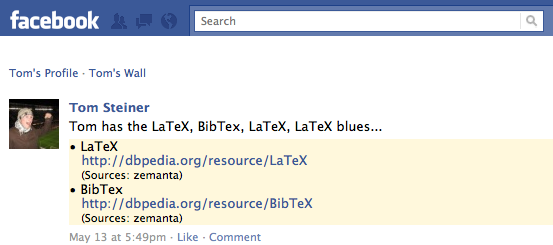
\includegraphics[width=0.45\textwidth]{facebook-swarm-nlp.png}
  \caption{Facebook Swarm NLP browser extension. Extracted named entities have a pale yellow background.}     
  \label{fig:facebook}
\end{figure}

\subsection{A Mash-up API for Named Entity Disambiguation}
As mentioned before, in order to perform named entity extraction and disambiguation, we rely on a mash-up API that calls existing third party NLP APIs in the background and that delivers the combined results of these APIs in a consolidated way. It is  desirable (i)~to credit back the contribution of each single third party API to the joint results, and (ii)~to track the provenance of the joint results in order to understand how they were formed. We will show at the concrete example of the mash-up NLP API used for our browser extension how these two constraints can be fulfilled in a generalizable way.

\subsection{Paper Structure}
The remainder of this paper is structured as follows: we discuss related work in Section~\ref{sec:related}. We show how unstructured data can be structured in Section~\ref{sec:structuring}. In Section~\ref{sec:consolidate}, we show how named entities from multiple sources can be consolidated. Section~\ref{sec:tracking} focuses on how data provenance can be tracked for combined mash-up APIs. Section~\ref{sec:conclusion} gives an outlook on future work and ends the paper with a conclusion. 

\section{Related Work}\label{sec:related}
We regard related work from different angles. First, we look into different approaches for named entity disambiguation, which is relevant for adding meaning to microposts.
Second, we look into efforts in mashing up Web services, which is important for tracking data provenance when using multiple APIs in combination.

\subsection{Entity Disambiguation Using Lexical Databases}
In~\cite{Choudhury:YouTube}, Choudhury \emph{et al.} describe a framework for semantic enrichment, ranking, and integration of
Web video tags using Semantic Web technologies. This task is more related to microposts as it seems like at a first glance: video tags can consist of more than one word, and microposts (on Twitter) oftentimes consist of just a few words by design. In order to enrich the typically sparse user-generated tag space, meta
data like the recording time and location, or the video title and video description are used, but also social features
such as playlists where a video appears in and related videos. Next, the tags are ranked by their co-occurrence and in
a final step interlinked to DBpedia concepts for greater integration with other
datasets. Choudhury \emph{et al.} disambiguate the tags based on WordNet~\cite{Princeton:WordNet} synsets if possible (\emph{i.e.}, if
there is only one matching synset in WordNet, the corresponding WordNet URI in DBpedia is selected. If there are more
than one matching synsets, the tags and their context tags similarity is computed and thereby tried to decide on an
already existing tag URI).
Lopez \emph{et al.} describe in~\cite{Lopez} an automatic titling method based on the four stages corpus 
acquisition, candidate sentences determination, noun 
phrase extraction, and selection of a particular noun phrase to play the role of the text title. Their method is in so far relevant to our work as automatically generated text titles can simplify the micropost annotation step for longer microposts, where annotated titles are used instead of the actual micropost.

\subsection{Entity Disambiguation With Semantic Coherence And News Trends}
In~\cite{Fernandez:IdentityRank}, Fern\'{a}ndez \emph{et al.} examine entity disambiguation in the context of news annotation.
They introduce a novel algorithmic approach to entity disambiguation called \textit{IdentityRank}. Running IdentityRank
on a news item consists of three steps: finding the candidate instances in the news ontology for each entity in the
news item, ranking these candidate instances using a modified version of PageRank~\cite{Brin:PageRank}, and finally
retraining the algorithm with the journalist's feedback once the process is finished. IdentityRank first takes into
account the number of occurrences of candidate entities in the past in order to find news trends, and second the
occurrences of candidate entities in past articles in the same categories in order to find semantic coherences.

\subsection{Disambiguation With Disambiguation Dictionaries}
In~\cite{Nguyen:NamedEntity}, Nguyen \emph{et al.} show how disambiguation dictionaries can be used to disambiguate entities
using disambiguation data extracted from Wikipedia, mostly based on Wikipedia 
disambiguation pages. For a set of entity 
candidates, all disambiguations are ranked using TF-IDF (or cosine similarity). The approach is a hybrid and incremental process that utilizes previously identified named
entities and related terms co-occurring with ambiguous names in a text for entity disambiguation.

\subsection{Disambiguation With Corpuses and Probability}
Cucerzan shows in~\cite{Cucerzan:Wikipedia} the use of a corpus like Wikipedia for entity disambiguation. The
surrounding words of the to-be-disambiguated terms plus the tags and categories of the related Wikipedia articles are
 used to determine semantic coherence and thus to decide on the most probable entity candidate. This happens
through a process of heuristically maximizing the agreement between contextual information extracted from Wikipedia and
the context of a document.

In~\cite{Sangeetha}, Sangeetha \emph{et al.} provide a framework that adds meaning to unstructured texts in the form of extracted events by combining three techniques, 
namely, statistical methods for identifying event triggers, 
text meaning representation for identifying thematic 
roles which map into event arguments, and rule based 
methods for event property identification.

\subsection{Disambiguation With Search Query Logs}
In~\cite{Billerbeck:QueryLogs}, Billerbeck \emph{et al.} use click graphs and session graphs of users' search engine sessions
to semantically bridge different queries in order to retrieve entities for a concrete entity retrieval query. Click
graphs are created by using queries and URLs as nodes and connecting and weighting them by their user click
frequencies. Session graphs are created by using only queries as nodes with edges between them if they appear in the same user
sessions, again weighted by co-occurrence frequencies. An exemplary entity retrieval query might be \textit{hybrid
cars}, semantically bridgeable queries might be \textit{toyota prius}, or \textit{honda civic hybrid}). These entities
are then ranked and returned to the user.

\subsection{Combining Different Web Services and Provenance}
In~\cite{Groth:2009:MPD:1462159.1462162}, Groth \emph{et al.} describe how through tools and technologies such as Yahoo! Pipes, Really Simple Syndication (RSS) and APIs, so-called mash-ups can be created in a dynamic, just-in-time way, combining data from different data sources. The authors are driven by the motivation to allow for trust and confidence in mash-ups, and therefore consider it critical to be able to analyze the origin of combined results. They suggest an approach based on OWL and XML, with a focus on process documentation. However, different from us, where the goal is to transparently add provenance data at API invocation level, their focus is more on overall process documentation in the context of a mash-up application.

The focus of Carroll \emph{et al.} in~\cite{carroll2005} is on the provenance of triples in the Semantic Web world, namely, for making statements about triples in graphs. Therefore, the paper introduces the concept of named graphs, an extension to RDF. In contrast to our work, Carroll \emph{et al.} focus purely on using triples to make statements about triples (\emph{i.e.}, stay in the RDF world), whereas our approach uses RDF to make statements about potentially any API result. In consequence, our approach is not limited to RDF results, albeit in the concrete case, we use RDF in addition to JSON as API result formats.
 
In the \emph{WS--*} world, BPEL4WS, described by Curbera \emph{et al.} in~\cite{Curbera:2003:NSW:944217.944234} provides a formal language for the specification of business processes and business interaction protocols. This allows for the combination of several APIs, however, it does not credit back concrete outputs of a combined API to the underlying APIs.

In~\cite{Yu}, Yu \emph{et al.} propose to apply Linked Data principles to expose 
Web services and Web APIs and introduce a framework in which 
service registries as well as services contribute to the automation 
of service discovery, and hence, workload  is distributed more 
efficiently. This is achieved by developing a Linked Data 
compliant Web services framework. This framework aims at 
optimizing load balance and performance by dynamically 
assembling services at run time in a massively distributed Web 
environment.
The authors' main goal is service discovery and orchestration, however, without a dedicated focus on providing provenance information for retrieved combined results.

\section{Structuring Unstructured Textual Data} \label{sec:structuring}
When we speak of adding structure to unstructured textual data we mean the process of extracting the main concepts in the form of named entities from a given text. An ``entity'' is defined by WordNet as ``that which is perceived or known or inferred to have its own distinct existence (living or nonliving)''. Typically named entities from a text can be persons, companies, organizations, geographies, but also things like quantities, expressions of time, books, albums, authors etc. The extraction is based on Natural Language Processing (NLP) and Machine Learning.

\subsection{Natural Language Processing Services}\label{sec:nlp-services}
Natural Language Processing is defined as ``the branch of information science that deals with natural language information''. From the many NLP toolkits, in the following we list some NLP Web services that link to datasets in the Linked Open Data
cloud\footnote{\textit{http://lod-cloud.net/}} in order to disambiguate named entities.

\subsection{OpenCalais}\label{sec:opencalais}
OpenCalais~\cite{OpenCalais} is the only Web service we use that provides details on occurrences in concrete sections of the submitted coherent text. This allows for exact matching of the location in the text where a certain entity is believed to appear. This is especially useful as OpenCalais is also oftentimes capable of recognizing references within the text to prior discovered entities (see the emphasized words as an example: ``\emph{Obama} thanked people for their work in ensuring the victory. \emph{He} also thanked his family […]''). An OpenCalais response consists of three parts:

\begin{itemize}
\item a list of topics that the text could be categorized in.
\item a list of concrete entities that occur in the text.
\item a list of social tags that a human being could assign.
\end{itemize}

The problem with the extracted entities is that they are not always disambiguated. An example is the URI \textit{http://d.opencalais.com/pershash-1/cf42394f-4ae9-3e8e-958a-088149c86565.html} that represents the concept of type ``person'' of president Barack Hussein Obama. However, president Barack Obama is also represented by the URI \textit{http://d.opencalais.com/pershash-1/cfcf1aa2-de05-3939-a7d5-10c9c7b3e87b.html} that was returned in one and the same response to one of our test requests. A second issue is that only a tiny fraction of the returned entities link to other Linked Open Data (LOD) sources in the LOD cloud. In order to find links to the linking hub DBpedia, each returned entity has to be retrieved at the expense of an HTTP request, and the returned RDF has to be checked for said links.

\subsection{AlchemyAPI}
AlchemyAPI~\cite{AlchemyAPI} differentiates between entities and concepts, however, in practice the difference being very subtle, we treat entities and concepts the same. Overall the AlchemyAPI results are very accurate and of mostly excellent Linked Data quality as there are links to well-known members of the LOD cloud, among others to DBpedia, OpenCyc, and Freebase. AlchemyAPI also provides links to other data sources, however, sometimes the returned URIs resolve to 404 ``Not found'' errors. One example that we came across during our tests was the URI \textit{http://umbel.org/umbel/ne/wikipedia/George\_W.\_Bush.rdf}, which should represent the concept of the person George W. Bush. AlchemyAPI also oftentimes returns thematically very related, but for a concrete text not directly relevant entities.

\subsection{Zemanta}
Zemanta~\cite{Zemanta} provides high quality entities that are linked to well-known datasets of the LOD cloud, \emph{e.g.}, DBpedia, Semantic CrunchBase, or Freebase. Zemanta convinces through very accurate entity disambiguation and thus high precision, however, at the cost of recall. Where other services try to return at least something of lower precision, the design objectives of Zemanta instead seem to prefer not to return anything if the underlying algorithms are unsure of the quality of the results. 

\subsection{DBpedia Spotlight}
DBpedia Spotlight~\cite{spotlight} is a tool for annotating mentions of DBpedia resources in text, providing a solution for linking unstructured information sources to the Linked Open Data cloud through DBpedia. DBpedia Spotlight performs named entity extraction, including entity detection and disambiguation with adjustable precision and recall.

\section{Consolidating Named Entity Disambiguation Results} \label{sec:consolidate}
In this section, we motivate the use of multiple existing named entity disambiguation Web services in parallel for the task of
obtaining entity candidates for a text such as a micropost. In addition to that, we also introduce the notion of
\texttt{owl:sameAs}-based approaches.

\subsection{Identity Links On the Semantic Web}                             \label{sec:sameasorg}
In order to tackle the problem of different namespaces in results that we have outlined before, a straightforward idea is to use a Web service such as
sameAs~\cite{Glaser:SameAs} to easily find mappings from one namespace into another. In practice,
however, while many data sources in the Linked Data world are marked as being equal to each other (\emph{e.g.},
\textit{http://dbpedia.org/resource/Barack\_Obama} \texttt{owl:sameAs} \textit{http://rdf.freebase.com/rdf/en.barack\_obama}),
the quality of such equality links is not always excellent. As Halpin \emph{et al.} show in~\cite{Halpin:SameAs}, the problem
with \texttt{owl:sameAs} is that people tend to use it very differently. The authors 
differentiate four separate usage styles, each with its particular implications. Inference is thus problematic, if not
impossible, when the sense of the particular use of \texttt{owl:sameAs} is unknown.

\subsection{Linked Data Principles Applied}
Sir Tim Berners-Lee has introduced Linked Data in a W3C Design Issue~\cite{TimBL:LinkedData}, where he defines the four rules for Linked~Data:
\begin{enumerate}
\item Use URIs as names for things.
\item Use HTTP URIs so that people can look up those names.
\item When someone looks up a URI, provide useful information, using the standards (RDF*, SPARQL).
\item Include links to other URIs, so that they can discover more things.
\end{enumerate}
In order to represent extracted named entities from social network microposts in an unambiguous way, we apply the first and the second Linked Data principle by representing named entities with HTTP URIs. This is taken care of by the third party NLP APIs that we use for our Chrome extensions, namely OpenCalais~\cite{OpenCalais}, Zemanta~\cite{Zemanta}, DBpedia Spotlight~\cite{spotlight}, and AlchemyAPI~\cite{AlchemyAPI}. These APIs take a text fragment as input, perform named entity extraction on it, and then link the extracted entities back into the Linking Open Data (LOD) cloud. We use these APIs in parallel, and by combining their results aiming at the emergence effect in the sense of Aristotle: ``\emph{[\ldots] the totality is not, as it were, a mere heap, but the whole is something besides the parts [\ldots]}''\footnote{Aristotle, Metaphysics, Book H 1045a 8-10.}. 

\subsection{Entity Consolidation Process}
We define the process of entity consolidation as the merging process of entities, \emph{i.e.}, if several services extract the same or different
entities from the same input text fragment or term, we say that the entity is consolidated if through entity ranking a winning entity has been determined.

The considered existing named entity disambiguation Web services (also referred to as entity mapping services) take as input parameter a text, and return a ranked list of entity
candidates, all identified by URIs, and enriched by depending on the service more or less meta information. In order to
gain confidence in a decision it is a common pattern to rely not only on the response from one source, but to
independently request responses from several sources. Figure~\ref{fig:diagram} illustrates this idea for four named entity disambiguation Web services. The figure has two levels: the direct result level that contains the direct output of the 
particular entity mapping service, and the \texttt{owl:sameAs} level that contains \texttt{owl:sameAs} results for the
direct results. These are obtained either from data in the direct result entities themselves, or from a Web service
like sameAs.org, described by Glaser \emph{et al.} in~\cite{Glaser:SameAs}.

\begin{figure*}
 \centering
 \vspace{2em}
 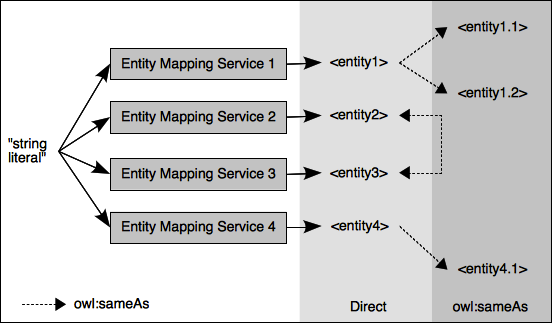
\includegraphics[width=0.6\textwidth]{diagram.png}
 \caption{Exemplary result set configuration using four entity mapping services with only the particular top result displayed for each entity mapping service. The figure shows the direct results of the particular entity mapping service, and \texttt{owl:sameAs} results for the direct results.}
 \label{fig:diagram}
\end{figure*}

In the following we will discuss strategies in order to decide for the most probable entity candidate from a given
result set configuration.

\subsection{Direct Approaches}
The most obvious class of approaches is what we call direct approaches, \emph{i.e.}, with direct approaches we do not look at potential \texttt{owl:sameAs} data at all, but exclusively work with the direct output of the entity mapping Web services.

\paragraph{Majority-based Winner Entity Determination}\label{sec:direct}
By \textit{majority-based} we mean that simply the entity with the most votes is elected the winner entity. If no
winner can be determined, we either randomly select a winner, or rank the candidates by the trustworthiness of the
particular Linked Data sources (a complete definition of \textit{trustworthiness of Linked Data sources} is out of
scope of this paper, however, the number of inbound links in the Linked Open Data
cloud is a good indicator).

We treat each of the first $n$ results of each service equally, and elect the winner entity by determining the
absolute majority of entities as in Subsection~\ref{sec:direct}. The chance to have a correct entity within all results is
higher the more results we consider. A next step different from treating each of the first $n$
results equally is to preserve the information of the entity mapping services' ranking by introducing rank
weights. The particular ranking formula of each entity mapping service is not necessarily known, however, we treat it as a black box and assume objective ranking criteria.

\paragraph{Direct Source-weighted Winner Entity Determination}
Another option is to always select the trustworthiest result by the inbound links ranking criteria as outlined in Section~\ref{sec:direct}, independent from the majority constellation. Practically speaking this means that
if, \emph{e.g.}, DBpedia is considered trustworthier as, \emph{e.g.},  GeoNames\footnote{\textit{http://www.geonames.org/}}, we
trust the DBpedia result over any other result from GeoNames.

\paragraph{Direct Majority-based Source-weighted Winner Entity Determination}
Based on direct majority-based winner entity determination we introduce weight factors that give trustworthy
sources a boost. This means that even if in a concrete instance a certain trustworthy source does not have the majority of votes, it still
can win the election and be the winning entity. The final result depends on the to-be-determined concrete
weight factors and on the particular majority constellation. Conflicts are be resolved as outlined in Section~\ref{sec:direct}.

\subsection{owl:sameAs Approaches}
With \texttt{owl:sameAs} approach, we mean that in addition to the direct results of the entity mapping Web services, we also
consider \texttt{owl:sameAs} data for the direct results.

\paragraph{owl:sameAs Majority-based Winner Entity Determination}\label{sec:owlsameas}
Analogue to direct majority-based winner entity determination, \texttt{owl:sameAs} majority-based winner entity
determination works by introducing entity clusters. An entity cluster is defined by a direct result and its
\texttt{owl:sameAs} corresponding sub-results. The entity cluster with the most votes is then elected as winning
cluster, \emph{i.e.}, the winner entity is the direct result of its particular winning entity cluster.

\paragraph{owl:sameAs Source-weighted Winner Entity Determination}
This approach is very similar to the corresponding direct approach, with the difference that a low-weight direct result
(direct in the sense of being a direct output of the entity mapping Web service) still wins if it has high-weight
\texttt{owl:sameAs} sub-results.

\paragraph{owl:sameAs Source-weighted Majority-based Winner Entity Determination}
Within entity clusters we apply source weights in order to emphasize trustworthy sources and then apply
majority-based winner determination as described in Section~\ref{sec:owlsameas}.

\subsection{Exemplary Entity Consolidation}                     \label{sec:consolidation-nlp}
We recall the mash-up API described in the introduction of this paper that calls third party NLP Web services in order to return a combined result of consolidated entities.
All NLP Web services return entities with their types and/or subtypes, names,
relevance, and URIs that link into the LOD cloud. The problem is that each service has implemented its own typing
system and providing mappings for all of them would be a relatively time-consuming task. However, as all services
provide links into the LOD cloud, the desired typing information can be pulled from there in a true Linked Data manner. The least common
multiple of the results for the query ``Google Translate'' is depicted below. For the sake of clarity, we just show one
entity with two URIs while the original result contained seven entities among which six were relevant and one was only loosely related.
\newpage
\begin{lstlisting}
[
  {
    "name": "Google Translate",
    "relevance": 0.7128319999999999,
    "uris": [
      {
        "uri": "http://dbpedia.org/resource/Google_Translate",
        "source": "alchemyapi"
      },
      {
        "uri": "http://rdf.freebase.com/ns/en/google_translate",
        "source": "zemanta"
      }
    ],
    "source": "alchemyapi,zemanta"
  }
]
\end{lstlisting}
\vspace{2em}

These results come from a request to our wrapper API via \texttt{GET} \textit{/entity-extraction/combined/Google\%20Translate},
and the particular services' results can be obtained via \texttt{GET} \textit{/entity-extraction/\{service\_name\}/Google\%20Translate\%20is\%20a\\\%20service\%20by\%20Google}.
While AlchemyAPI and Zemanta return results from DBpedia and other interlinked LOD cloud resources, OpenCalais returns
only results in its own namespace
(\emph{e.g.}, \nofootnote{\textit{http://d.opencalais.com/er/company/ralg-tr1r/ce181d44-1915-3387-83da-0dc4ec01c6da.rdf}} for the
company Google). In this particular case, retrieving the resource RDF representation and parsing for
\texttt{owl:sameAs} return links to DBpedia. However, in the general case, we found OpenCalais URIs sometimes pointing
to non-existent resources or to not very rich resources such
as\nofootnote{\textit{http://d.opencalais.com/pershash-1/cfcf1aa2-de05-3939-a7d5-10c9c7b3e87b.html}}, a URI identifying
the current US President Barack Obama where the only information is that Barack Obama is of type person. In order to
consolidate extracted entities, we use the following approach: we have a look at each of the extracted entities from
service one and compare each entity's URIs with each URIs from each extracted entity from service two, illustrated below.

First, we consider the isolated results for the text fragment from AlchemyAPI only:
\vspace{2em}
\begin{lstlisting}
{
  "name": "Google",
  "relevance": 0.496061,
  "uris": [
    {
      "uri": "http://dbpedia.org/resource/Google",
      "source": "alchemyapi"
    },
    {
      "uri": "http://rdf.freebase.com/ns/guid.9202a8c04000641f800000000042acea",
      "source": "alchemyapi"
    },
    {
      "uri": "http://cb.semsol.org/company/google.rdf",
      "source": "alchemyapi"
    }
  ],
  "source": "alchemyapi"
}
\end{lstlisting}
\vspace{2em}
Second, we consider the isolated results for the same text fragment from Zemanta only:
\newpage
\begin{lstlisting}
{
  "name": "Google Inc.",
  "relevance": 0.563132,
  "uris": [
    {
      "uri": "http://rdf.freebase.com/ns/en/google",
      "source": "zemanta"
    },
    {
      "uri": "http://dbpedia.org/resource/Google",
      "source": "zemanta"
    },
    {
      "uri": "http://cb.semsol.org/company/google#self",
      "source": "zemanta"
    }
  ],
  "source": "zemanta"
}
\end{lstlisting}
\vspace{2em}
Finally, we consider the merged results from both Zemanta and AlchemyAPI. Note that these results are not exposed externally, they are used internally by the wrapper Web service:
\vspace{2em}
\begin{lstlisting}
{
  "name": [
    "Google",
    "Google Inc."
  ],
  "relevance":  0.5295965,
  "uris": [
    {
      "uri": "http://dbpedia.org/resource/Google",
      "source": "alchemyapi"
    },
    {
      "uri": "http://rdf.freebase.com/ns/guid.9202a8c04000641f800000000042acea",
      "source": "alchemyapi"
    },
    {
      "uri": "http://umbel.org/umbel/ne/wikipedia/Google",
      "source": "alchemyapi"
    },
    {
      "uri": "http://cb.semsol.org/company/google.rdf",
      "source": "alchemyapi"
    },
    {
      "uri": "http://rdf.freebase.com/ns/en/google",
      "source": "zemanta"
    },
    {
      "uri": "http://cb.semsol.org/company/google#self",
      "source": "zemanta"
    }
  ],
  "source": "alchemyapi,zemanta"
}
\end{lstlisting}
\vspace{2em}
In this example, the entity names mismatch (``google inc.'' vs. ``google''). However, going down the list of URIs for
the entity, one can note a match via\nofootnote{\textit{http://dbpedia.org/resource/Google}}. Additionally, there can also
be seen two would-be matches: \nofootnote{\textit{http://cb.semsol.org/company/google.rdf}}
vs.\nofootnote{\textit{http://cb.semsol.org/company/google\#self}} and
\nofootnote{\textit{http://rdf.freebase.com/ns/en/google}} vs.
\nofootnote{\textit{http://rdf.freebase.com/ns/guid.9202a8c04000641f80000000\\0042acea}}. However, the inconsistent use of
URIs when there are more than one URIs available for the same entity hinders the match from being made. An additional
retrieval of the resources would be necessary to detect that in the latter case
\nofootnote{\textit{http://rdf.freebase.com/ns/guid.9202a8c04000641f80000000\\0042acea}} redirects to
\nofootnote{\textit{http://rdf.freebase.com/ns/en/google}}, whereas the first example seems to be broken
(\nofootnote{\textit{http://cb.semsol.org/company/google\#self}} returns the status code 404). The good thing, however, is
that as soon as \emph{one} match has been detected, one can consolidate the entities from both services.

Given the mismatching two entity names (``google inc.'' vs. ``google''), the consolidated name is then an array of all
detected synonymous. The consolidated relevance is the average relevance of both services. Each service already includes a relevance score ranging from
0 (irrelevant) to 1 (relevant), so we directly use it. In our approach, the consolidated and merged entities from
service one and two are then in turn compared to extracted entities from service three and so on, if we used even more
services. In practice, however, due to the not always given interconnectedness of OpenCalais, there are no matches
after having compared Zemanta-extracted entities with AlchemyAPI-extracted entities. We maintain provenance metadata for each URI on the lowest data representation level (JSON)
on both a per URI basis and an entity basis with the NLP-detected entity consolidation.

\section{Tracking Provenance With Multiple Sources}                    \label{sec:tracking}
As outlined before, we use several data sources (APIs) in the background in order to add meaning to social network microposts. Extracted named entities from a micropost might in consequence be the result of up to four agreeing (or disagreeing) API calls. 

\subsection{The Need for Providing Provenance Metadata}
Hartig \emph{et al.} mention in~\cite{ipaw10:olaf} some reasons that justify the need for provenance metadata. Among those is linked dataset replication and distribution on the Web with not necessarily identical namespaces: based on the same source data, different copies of a linked dataset can be created with different degrees of interconnectedness by different publishers.

We add to this list the automatic conversion of legacy unstructured data to Linked Data with heuristics where extracted entities---while being consolidated and backed up by different data sources---might still be wrong. Especially with our ``mash-up''-like approach, it is very desirable to be able to track back to the concrete source where a certain piece of information comes from. This enables (i) to correct the error at the root of our API (fighting the cause), (ii) to correct the concrete error in an RDF annotation (fighting the symptom), and (iii) to judge the trustworthiness and quality of a dataset, which is probably the most important reason.

In order to track the contributions of the various sources, we have decided to use the Provenance Vocabulary~\cite{Hartig:Provenance} by Hartig and Zhao with the prefix \texttt{prv}, the HTTP Vocabulary in RDF~\cite{HTTP:RDF} by Koch \emph{et al.} with prefix \texttt{http}, and a vocabulary for Representing Content in RDF~\cite{CNT:RDF} by the same authors with prefix \texttt{cnt}. We have chosen the HTTP Vocabulary in RDF for the fact that it is a W3C Working Draft  developed by the Evaluation and Repair Tools Working Group (ERT WG), which is part of the World Wide Web Consortium (W3C) Web Accessibility Initiative (WAI). The Provenance Vocabulary was chosen because of its relatively broad implementation in several projects, such as Pubby\footnote{\texttt{http://www4.wiwiss.fu-berlin.de/pubby/}}, Triplify\footnote{\texttt{http://triplify.org/Overview}}, and D2R Server\footnote{\texttt{http://www4.wiwiss.fu-berlin.de/bizer/d2r-server/}}.

While our mash-up API supports two output formats (application/json and text/turtle), we have added provenance information exclusively to the text/turtle variant. In order to represent the extracted named entities in a micropost, we use the Common Tag vocabulary~\cite{CommonTag:Spec}. A micropost is \texttt{ctag:tagged} with a \texttt{ctag:Tag}, which consists of a textual \texttt{ctag:label} and a pointer to a resource that specifies what the label \texttt{ctag:means}. The Common Tag vocabulary is well-established and developed by both industry and academic partners. In order to make statements about a bundle of triples, we group them in a named graph. We use the TriG~\cite{Bizer:TriG} syntax:
\vspace{2em}
\begin{lstlisting}
:G = {
  <https://www.facebook.com/Tomayac/posts/10150175940867286> ctag:tagged [
      a ctag:Tag ;
      ctag:label "BibTeX" ;
      ctag:means <http://dbpedia.org/resource/BibTeX>
    ] .
} .
\end{lstlisting}

\subsection{The Provenance Vocabulary}                                      \label{sec:provenance}
In this section, we outline the required steps in order to make statements about the provenance of a group of triples contained in a named graph \texttt{:G} that was generated using several HTTP \texttt{GET} requests to third party APIs. We use the Provenance Vocabulary~\cite{Hartig:Provenance} with prefix \texttt{prv}, the HTTP Vocabulary in RDF~\cite{HTTP:RDF} with prefix \texttt{http}, and the Representing Content in RDF~\cite{CNT:RDF} vocabulary with prefix \texttt{cnt}.

First, we state that \emph{:G} is both a \emph{prv:DataItem} and obviously an \emph{rdfg:Graph}. \emph{:G} is \emph{prv:createdBy} the process of a \emph{prv:DataCreation}. This \emph{prv:DataCreation} is \emph{prv:performedBy} a \emph{prv:NonHumanActor}, a \emph{prvTypes:DataProvidingService} to be precise (simplified as \emph{http://tomayac.no.de/entity-extraction/combined} in the listing). This service is \emph{prv:operatedBy} a human (\texttt{http://tomayac.com/thomas\_steiner.rdf\#me}). Time is often important for provenance, so the \emph{prv:performedAt} date of the \emph{prv:DataCreation} needs to be saved. During the process of the \emph{prv:DataCreation} there are \emph{prv:usedData}, which are \emph{prv:retrievedBy} a \emph{prv:DataAcess} that is \emph{prv:performedAt} a certain time, and \emph{prv:performedBy} a non-human actor (our API) that is \emph{prv:operatedBy} a human (\texttt{http://tomayac.com/thomas\_steiner.rdf\#me}. For the \emph{prv:DataAccess} (there is one for each third party API involved), we \emph{prv:accessedService} from a \emph{prv:DataProvidingService} of which we \emph{prv:accessedResource} at a certain \emph{irw:WebResource}. Therefore, we \emph{prvTypes:exchangedHTTPMessage} which is an \emph{http:Request} using \emph{http:httpVersion} ``1.1'' and the \emph{http:methodName} ``GET''.

\subsection{Provenance RDF Overview}                                           \label{sec:appendix}
This section provides a shortened overview of the provenance RDF in Turtle syntax for a  micropost tagged with the label ``BibTeX'' and the assigned
meaning \texttt{http://dbpedia.org/resource/BibTeX}. The named graph \texttt{:G} in the first part of the listing contains the absolute data (the fact that the  micropost with the URI \texttt{https://www.facebook.com/Tomayac/posts/\-10150177486072286} is tagged with the label ``BibTeX'', which is represented by the HTTP URI \texttt{http://dbpedia.org/resource/BibTeX}). The second part with metadata about \texttt{:G} says that these facts were generated via two calls, one using the HTTP method \texttt{GET}, and the other \texttt{POST}.
It is to be noted that statements such as in the listing above refer to the triple objects as an identifier for a Web resource (where the Web resource is a representation of the result of the API call at the time where it was \texttt{prv:performedAt}). As provenance metadata always refers to the time context in which a certain statement was made, it is essentially unimportant what representation the resource returns in future.
\vspace{2em}
\begin{lstlisting}
:G = {
  <https://www.facebook.com/Tomayac/posts/10150177486072286> ctag:tagged [
     a ctag:Tag ;
     ctag:label "BibTeX" ;
     ctag:means <http://dbpedia.org/resource/BibTeX> ;
  ] .
} .


:G
  a prv:DataItem ;
  a rdfg:Graph ;
  prv:createdBy [
    a prv:DataCreation ;
    prv:performedAt "2011-05-20T15:06:30Z"^^xsd:dateTime ;
    prv:performedBy <http://tomayac.no.de/entity-extraction/combined> ;
    prv:usedData [
      prv:retrievedBy [
        a prv:DataAcess ;
        prv:performedAt "2011-05-20T15:06:30Z"^^xsd:dateTime ;
        prv:performedBy <http://tomayac.no.de/entity-extraction/combined> ;
        prv:accessedService <http://spotlight.dbpedia.org/rest/annotate> ;
        prv:accessedResource <http://spotlight.dbpedia.org/rest/annotate?text=Tom%20has%20the%20LaTeX%2C%20BibTeX%2C%20LaTeX%2C%20LaTeX%20blues...&confidence=0.4&support=20> ;
        prvTypes:exchangedHTTPMessage [
          a http:Request ;
          http:httpVersion "1.1" ;
          http:methodName "GET" ;
          http:mthd <http://www.w3.org/2008/http-methods#GET> ;
        ] ;
      ] ;
    ] ;
    prv:usedData [
      prv:retrievedBy [
        a prv:DataAcess ;
        prv:performedAt "2011-05-20T15:06:41Z"^^xsd:dateTime ;
        prv:performedBy <http://tomayac.no.de/entity-extraction/combined> ;
        prv:accessedService <http://api.zemanta.com/services/rest/0.0/> ;
        prv:accessedResource <http://api.zemanta.com/services/rest/0.0/> ;
        prvTypes:exchangedHTTPMessage [
          a http:Request ;
          http:httpVersion "1.1" ;
          http:methodName "POST" ;
          http:mthd <http://www.w3.org/2008/http-methods#POST> ;
          http:headers (
            [
              http:fieldName "Content-Type" ;
              http:fieldValue "application/x-www-form-urlencoded" ;
            ]   
          )
          http:body [
            a cnt:ContentAsText ;
            cnt:characterEncoding "UTF-8" ;
            cnt:chars """method=zemanta.suggest_markup
            &api_key=Your_API_Key
            &text=Tom%20has%20the%20LaTeX%2C%20BibTeX%2C%20LaTeX%2C%20LaTeX%20blues...
            &format=json
            &return_rdf_links=1""" ;
          ] ;
        ] ;
      ] ;
    ] ;
  ] .
\end{lstlisting}
\vspace{1.0em}
\section{Future Work and Conclusion}                                                        
\label{sec:conclusion}
In this paper, we have shown how the Provenance
Vocabulary can be used to keep track of the original third party Web service calls that led to the consolidated
results. These references to the original calls are to be understood as the identification of Web resources (\emph{i.e.}, the
results of a request). We have shown how a concrete multi-source Web service can automatically maintain provenance
metadata, both for entirely machine-generated content, but also for partly (or completely) human-generated content. We
believe that being able to track back the origin of a triple is of crucial importance, especially given the network
effect which is one of the Linked Data benefits. The generated triples are very verbose, and in consequence stating even simple facts that a combined result is based on two separate sub-results takes up a lot of space. The verbosity is mainly due to the used vocabularies, the Provenance Vocabulary and the HTTP Vocabulary in RDF.
Already commenced future work will be to explore ways to stick to existing standards as these vocabularies on the one hand, but on the other hand to simplify drastically in order to come to less verbose provenance descriptions. While it is always easier to come up with a specialized vocabulary that does one task well (for example we could imagine a simple vocabulary with the sole purpose to log the API call of a Web service invocation), broader reuse and acceptance can be gained by reusing existing vocabularies. We will see how to find the right balance here, and are conscious that our current approach is a first step in that direction, however, that many more steps are ahead to take. Our vision is to establish a common method for specifying provenance data for mash-up Web services. 

% use section* for acknowledgement
\section*{Acknowledgments}
T. Steiner is partially supported by the European Commission under Grant No. 248296 FP7 I-SEARCH project. J. Gabarr\'o is partially supported by TIN-2007-66523 (FORMALISM) and SGR 2009-2015 (ALBCOM). 
R. Verborgh is funded by Ghent University, the Interdisciplinary Institute for Broadband Technology, the Institute for the Promotion of Innovation by Science and Technology in Flanders, the Fund for Scientific Research Flanders, and the EU.
\newpage
\bibliographystyle{abbrv}
\bibliography{nwesp2011}

\vspace{5mm}

\noindent{\bf\Large Author Biographies} \vspace{5mm}

\textbf{Thomas Steiner}
Thomas Steiner is a proud dad-of-two, a Research Scientist at Google, and a PhD student at UPC.edu. His main research interests these days are the Semantic Web, Linked Data, and the architectural style REST. He holds two Master of Computer Science degrees, one from the Technical University of Karlsruhe, Germany, and the other from the École Nationale Supérieure d'Informatique et de Mathématiques Appliquées de Grenoble, France.

\vspace{4mm}

\textbf{Ruben Verborgh}
Ruben Verborgh received his Master degree in Computer Science Engineering from Ghent University, Belgium in 2010. He is a researcher with the Multimedia Lab — Ghent University, Department of Electronics and Information Systems (ELIS) and the Interdisciplinary institute for BroadBand Technology (IBBT). His interests include Semantic Web technologies, multimedia annotation, artificial intelligence and their relation to multimedia processing. Currently, he is working on moving multimedia algorithms to the Web and related issues, like semantic service descriptions.

\vspace{4mm}

\textbf{Joaquim Gabarró Vallés}
Joaquim Gabarro, was born in Barcelona (Spain) in 1953 and studied Physics and Computer Science, obtained his Ph.D.
from Universitat Politècnica de Catalunya in 1983. From 1985 is Associate Professor (Profesor Titular) in Universitat Politècnica de Catalunya. Currently represents
Spain in the TC1 (Foundations of Computer Sciences) of IFIP. Main research topics
are Concurrency, Complexity and
Web algorithms.

\vspace{4mm}

\textbf{Rik Van de Walle}
Rik Van de Walle received his M.Sc. and PhD degrees in Engineering from Ghent University, Belgium in 1994 and 1998 respectively. After a visiting scholarship at the University of Arizona (Tucson, USA), he returned to Ghent University, where he became professor of multimedia systems and applications, and head of the Multimedia Lab. His current research interests include multimedia content delivery, presentation and archiving, coding and description of multimedia data, content adaptation, and interactive (mobile) multimedia applications.

\end{document}
